% This file has been cloned from: http://www.github.com/Micket/chalmers

\RequirePackage[l2tabu,orthodox]{nag} % This package helps prevent you from doing things wrong.

% change doctorate to licentiate if necessary
\documentclass[licentiate,g5paper,gu]{chalmers-thesis}
% All options are; doctorate, licentiate, masters, bachelors, techreport,
% projectreport, nocover, draft, g5paper, and everything the standard report
% class support.

\usepackage{ifluatex} % Automatic check for luatex.
\usepackage[utf8]{inputenc} % File encoding, you should try to stick to utf8.
\usepackage{microtype} % Magically improves typesetting for pdflatex
%\usepackage{subfiles} % Convenient use of subfiles in documents. Using \subfile is optional. See README
\usepackage[swedish, english]{babel}

\usepackage{csquotes} % Needed for biblatex
\usepackage[%
    url=true
  , style=numeric%alphabetic%authoryear
  , maxbibnames=10%
  , maxcitenames=2%
  , mincitenames=1%
  , backref=true%
%  , dashed=false%
  , backend=biber%
  ] {biblatex} % Modern bibliography facilities (you may change style to numeric). Change to old bibtex if you insist on using that.
\usepackage[%
    pdftex%
  , hidelinks%
  , linktoc=all%
  , unicode%
  , bookmarksopen=true%
  , bookmarksopenlevel=0%
  , bookmarksnumbered=true%
  ]{hyperref} % links in pdf document
\usepackage{mathtools} % All your math related needs
\usepackage{tikz} % Draw figures. Required for cover page
%\usepackage{natbib}
\usepackage{fancyhdr} % fine-tuning of headers
\pagestyle{fancy}

% Read the manuals for the respective package to see the usage;
\usepackage{pdfpages} % For included other pdf files (like articles).
%\usepackage{thmtools} % For theorems.
%\usepackage{algorithms} % For algorithms.
\usepackage{listings} % For source code.
%\usepackage{booktabs} % High quality tables.
%\usepackage{siunitx} % For all your numerical values and units.
%\usepackage{pgfplots} % Make plots directly in latex. Also tables. Excellent package.
\usepackage{subfiles}
\usepackage{subcaption}
\usepackage{afterpage}% for "\afterpage"
\usepackage{xcolor}
\usepackage{pagecolor}% With option pagecolor={somecolor or none}
%\usepackage{subfig}
\usepackage{mhaskell}
%\usepackage{yourcustomcommands} % Put your custom commands in a file 'yourcustomcommands.sty' and load it like this.

% ???
\usepackage[page,toc]{appendix}

\usepackage{lipsum}\setlipsumdefault{1-3} % Package used to put in placeholder text. Remove it.

% User commands
\title{A Functional Approach to Hardware Software Co-Design.}
\author{Markus Aronsson} % Not common with more than one author
\thesisin{}
\department{Department of Computer Science and Engineering}
% \division{Division of Solid Mechanics}
\reportno{2018:184L}
% ISSN : 1652-876X
% \ISBN{123-21332-13423-123} % Only for doctorate
\copyrightyear{2018}

\opponent{
Dr.~Alban\\
Department of Computers\\
University of Somewhere\\
Sweden
}

\oppositiondate{10.00 am, 16\textsuperscript{th} Oct, 2018 in HA2 Hörsalsvägen 4, Göteborg}

% You should scale the figure according to textwidth and or paperheight.
\coverfigure{\scalebox{-1}[1]{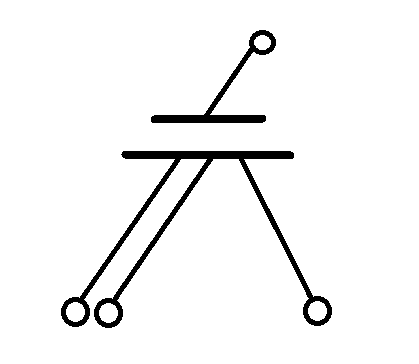
\includegraphics[width=\textwidth,height=0.4\paperheight,keepaspectratio]{figures/Cover}}}

% \covercaption{}

\firstabstract{
Developing software for embedded systems presents quite the challenge---not only do these systems demand good knowledge of the hardware they run on, but their limited resources also make it difficult to achieve efficiency. For embedded systems with different kinds of processing elements, the challenge is even greater; the presence of heterogeneous elements both raises all of the issues associated with homogeneous systems, and may also cause non-uniform system development and capability.

In this thesis we explore a functional approach to heterogeneous system development, with a staged hardware software co-design language embedded in Haskell, to address many of the modularity problems typically found in such systems. This staged approach enables designers to build their applications from reusable components and skeletons, while retaining control over much of the generated source code. Design exploration also benefits from the functional approach, since Haskell's type classes can be used to ensure that certain operations will be available. As a result, a developer can not only write for hardware and software in the co-design language, but she can also write generic programs that are suitable for both.

Internally, the co-design language is based on a monadic representation of imperative programs that abstracts away from its underlying statement, expression, and predicate types by establishing an interface to their respective interpreters. Programs are thus loosely coupled to their underlying types, giving a clear separation of concerns. The compilation process is expressed as a series of translations between progressively smaller typed languages, which safeguards against many common errors.

In addition to the hardware software co-design language, this thesis also introduces a language for expressing digital signal processing algorithms, using a model of synchronous data-flow that is embedded in Haskell. The language supports definitions in a functional style, reducing the gap between an algorithm's mathematical specification and its implementation. A vector language is also presented, which builds on a functional representation that guarantees fusion for arrays. Both of these languages are intended to be extensions of the co-design language, but neither one is dependent on it and can thus be used to extend other languages as well.
}

\keywords{functional programming, domain specific languages, signal processing, code generation}

\acknowledgements{
To my dearest, my fianc\'ee Emma Bogren: because I owe it all to you.

My constant cheerleaders, that is, my parents Dag and Lena: I am forever grateful for your moral and emotional support, you were always keen to know what I was doing and how I was proceeding. Although I'm fairly certain you never fully grasped what my work was all about, you never wavered in your encouragement and enthusiastic inquires. I am also grateful to my sibling Caroline who have supported me along the way, and her wonderful dog Alfons whom never failed to brighten my day.

A very special gratitude goes out to my advisor Mary Sheeran, for your continuous help and support in my studies, for your never ending patience, guidance and immense knowledge. With a special mention to my former co-worker Emil Axelsson, without your precious support I would not have been able to conduct my research. I will always miss our interesting and long-lasting chats.

I am also grateful to Anders Persson, Josef Svenningsson and Koen Claesson for their unfailing support and assistance. Your hard work, ideas and insights in the Feldspar project have proved a great source of inspiration in my research. Finally I express my gratitude to all my other colleagues at Chalmers, who make this a fantastic place to work.

Thank you all for your encouragement!
}

\paperwork{
Paper A introduces my signal processing language and an early version of our compilation techniques. I am the lead author but Emil Axelsson wrote the majority of sections 3.1 and 3.2. The paper was awarded the Peter Landin award for best paper at the \textit{International Symposium on Implementation and Applications of Functional Languages, IFL 2014}

Paper B introduces my hardware software co-design language and a mature version of our compiler and representation of imperative programs. The techniques presented are however not restricted to hardware software co-design, and can be of use for developers of embedded languages in general. I am the lead author.
}

% \secondabstract{swedish}{\lipsum} % Optional
% \preface{\lipsum} % You can use \input to put preface and acknowledgments in another document

% You can add extra contents such as abbreviations and nomenclature using.
% Use \presectiontitle to render add titles to new sections.
% \extrafrontmatter{\presectiontitle{Nomenclature} \lipsum} % Optional

% Other optional settings for biblatex;
\DeclareFieldFormat[article]{title}{#1} % Removes quotes from article title
\DeclareFieldFormat[article]{volume}{\mkbibbold{#1}} % Makes volume print in bold.
\renewbibmacro{in:}{} % Removes the "In:" from the journals field.
\DeclareFieldFormat[article]{pages}{#1} % Removes the pp. before pages.
% Adds short journal entries;
\renewbibmacro*{journal+issuetitle}{%
  \usebibmacro{shortjournal}%
  \setunit*{\addspace}%
  \iffieldundef{series}{}{\newunit\printfield{series}\setunit{\addspace}}%
  \usebibmacro{volume+number+eid}%
  \setunit{\addspace}%
  \usebibmacro{issue+date}%
  \setunit{\addcolon\space}%
  \usebibmacro{issue}%
  \newunit}
% End of optional citation modifications.

\addbibresource{library.bib} % New command, use if available
%\bibliography{library} % Legacy command

% \setlength{\topcolumn}{0.22\textwidth} % Column for "Thesis" page which might need adjustments if there is other publications.

\begin{document}
% \makethesisdefence % Should be printed at a5paper size
% \end{document}
\maketitle
% If you need to do any modifications, you can redefine each page respectively, or just call them manually as;
%\makecoverpage
%\maketitlepage
%\makeprintinfopage
%\makesecondabstractpage
%\makededicationpage
%\makeprefacepage
%\makeacknowledgementspage
%\maketableofpaperspage
%\cleardoublepage\tableofcontents
%\cleardoublepage\pagenumbering{arabic}

\part{Extended Summary} % Using the starred command avoids numbering.
\cleardoublepage

\subfile{kappa/introduction}
\subfile{kappa/background}
\subfile{kappa/codesign}
\subfile{kappa/results}

\begin{appendices}
\chapter{Synthesizing in Vivado}
\label{vivado}

This section explains the processes of manually importing and synthesizing a design in the 2015.2 version of Vivado~\cite{feist2012}. As this processes is the same for all designs, the explanation will focus on the required steps in a general sense rather than showcase a specific example.

Having generated code for a hardware program wrapped in the AXI4-lite interconnect, the first step is loading the code into a Vivado project. In the case of AXI4 projects, Vivado provides a wizard to create an AXI4 template under the  ``Create and Package IP'' action under ``Tools'' in the project's menu---the base project is typically supplied by the system's manufacturer, otherwise a basic one can be created by Vivado.

The AXI4 wizard will ask for a name, organization, and a few other details that are largely irrelevant to the template it generates, only the name is important as it will identify the component once it has been packaged. Afterward, the wizard will ask for a few settings, such as the number and size of its slave registers, these are again irrelevant and will be replaced later on. Once the wizard is finished the template can be added to the project's IP catalog and opened in an editing session, which should contain two files as shown in Figure~\ref{fig:files}.

\begin{figure}[h]
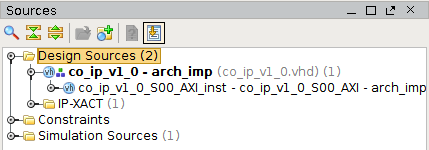
\includegraphics[width=0.4\textwidth]{figures/DesignFiles}
\centering
\caption{} % Design files generated for a AXI4 peripheral.
\label{fig:files}
\end{figure}

The first file in Figure~\ref{fig:files} simply contains a shell entity that instantiates a few constants an calls the empty AXI4-lite slave, which is located in the second file. Its this empty slave that should be substituted by the generated code. Note that, after updating the second design file the references from the first design file needs to be updated as well, since the slave's name most likely changed. Once that has been taken care of, the project can be reviewed and packaged---the review will probably complain that an address port has changed in size, as it always use the full 32 bits rather than a subset like Vivado. Go ahead and update its size accordingly.

Once the AXI4 peripheral has been updated, saved, and packaged, the main project can incorporate it as an ``IP Core'' in a few steps. Firstly, under the ``IP Settings'' menu, there is an option to locate the peripheral's project as a repository and to add its contents to the available IP cores. The component can the be added from either the context menu or from simply right-clicking the block design window and picking the option ``Add IP''. Vivado is able to connect the peripheral automatically to the main project by running its ``Run Connection Automation'' tool---Vivado will typically prompt for this option once an IP has been added. Figure~\ref{fig:system} shows the block design view of an example for a Parallell project that has been stripped to the bare minimum of components (a Zynq with a few components for managing AXI4 peripherals), where the AXI4-lite slave is the smaller box in the lower right of the view. Note that it is possible to get the physical address of the slave from the ``Address Editor'' at this point.

\begin{figure}[h]
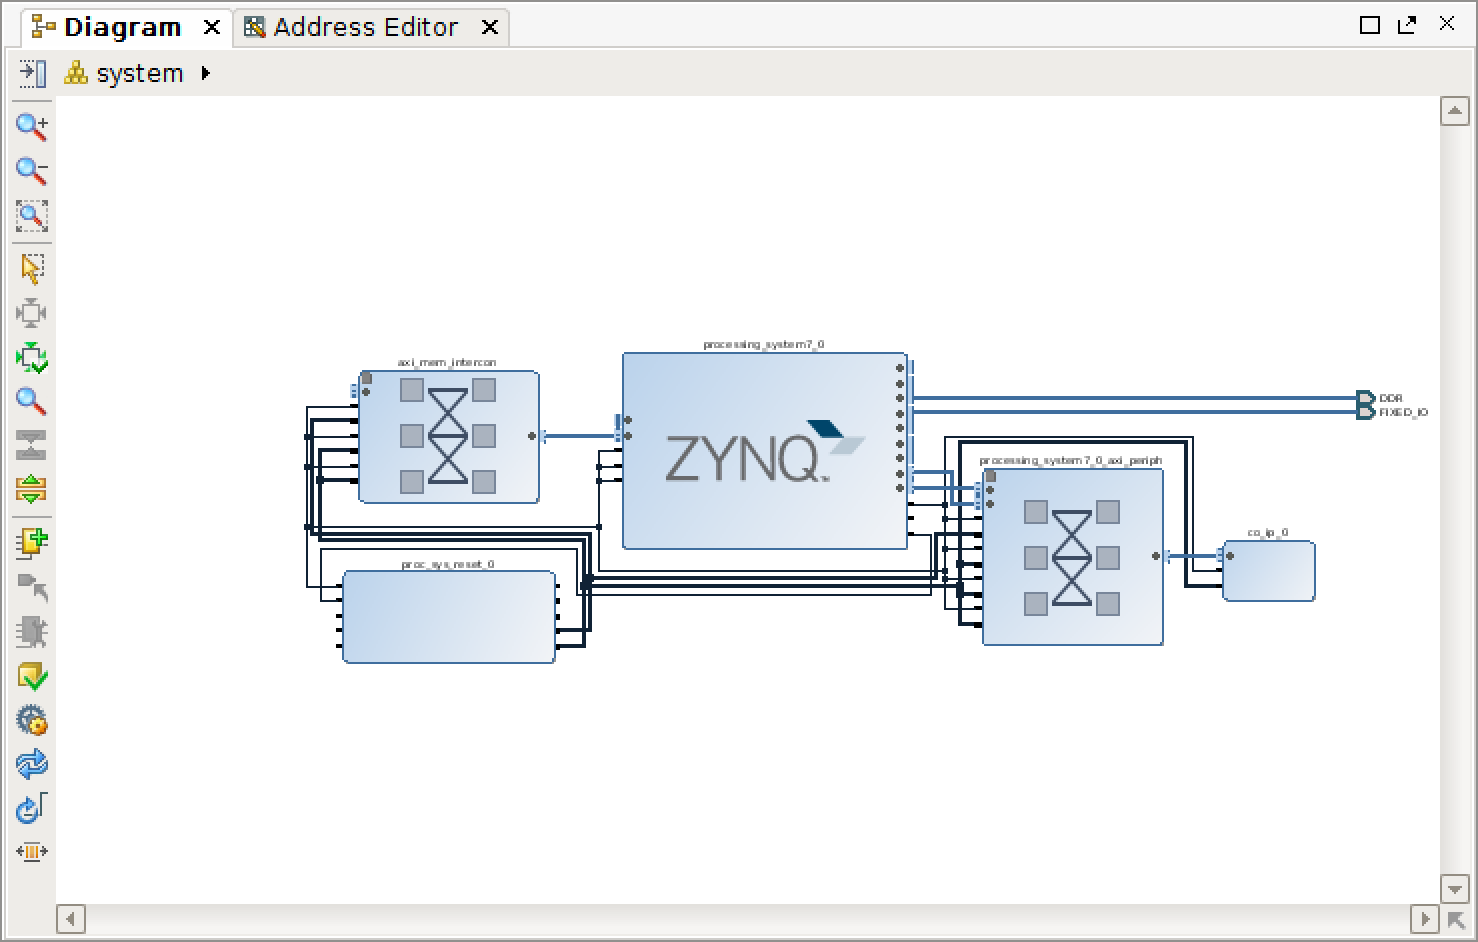
\includegraphics[width=0.4\textwidth]{figures/ZynqSystem}
\centering
\caption{} % Zynq project with AXI4-lite peripheral.
\label{fig:system}
\end{figure}

Finally, the last step is to generate a bitstream that flashed onto the FPGA's programmable logic. The project's context menu provides an action for generating the bitstream, and with the example project from Figure~\ref{fig:system}, produces an implementation like the one in Figure~\ref{fig:design}.

\begin{figure}[h]
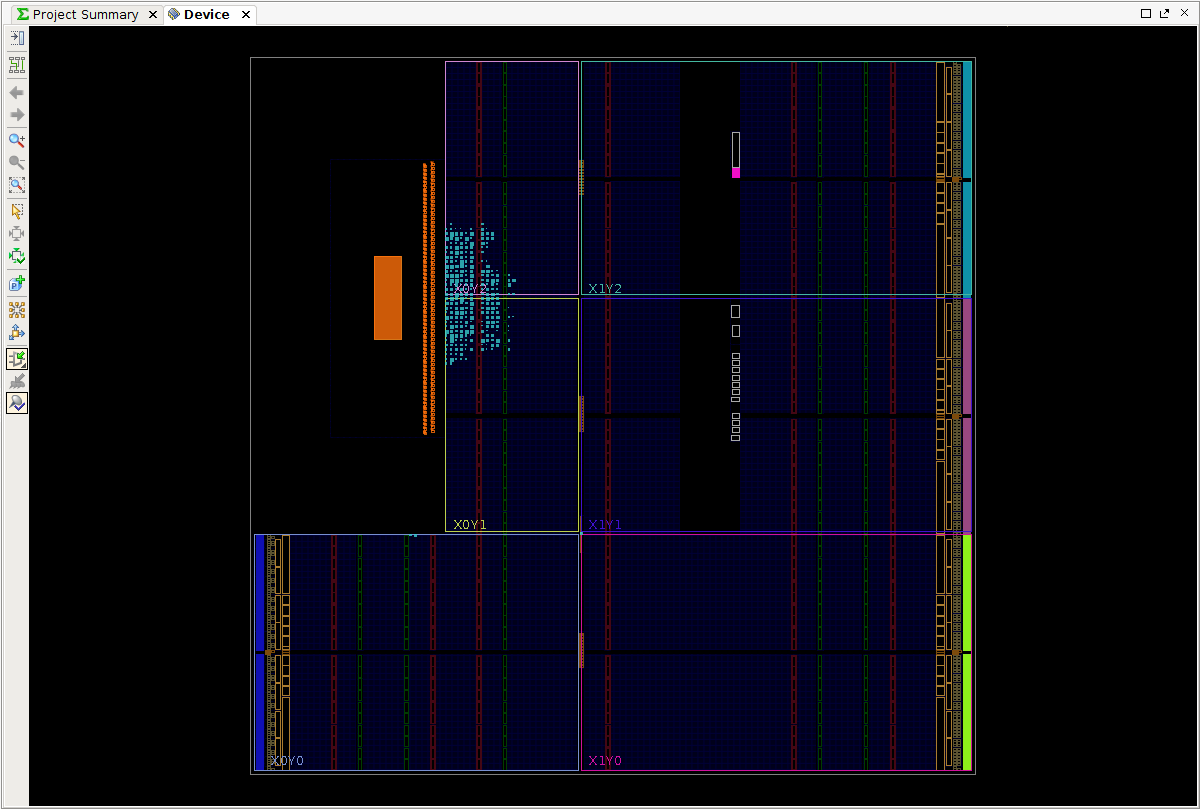
\includegraphics[width=0.4\textwidth]{figures/ZynqDesign}
\centering
\caption{Implementation of the project.}
\label{fig:design}
\end{figure}

\end{appendices}

\clearpage

\nocite{*} % Cites everything from the bibliography
\printbibliography % This command is new in biblatex. Do not attempt to use style files as with old latex.

\part{Appended Papers}
\cleardoublepage

\paper{\citefield{aronsson2014}{title}}{\fullcite{aronsson2014}}
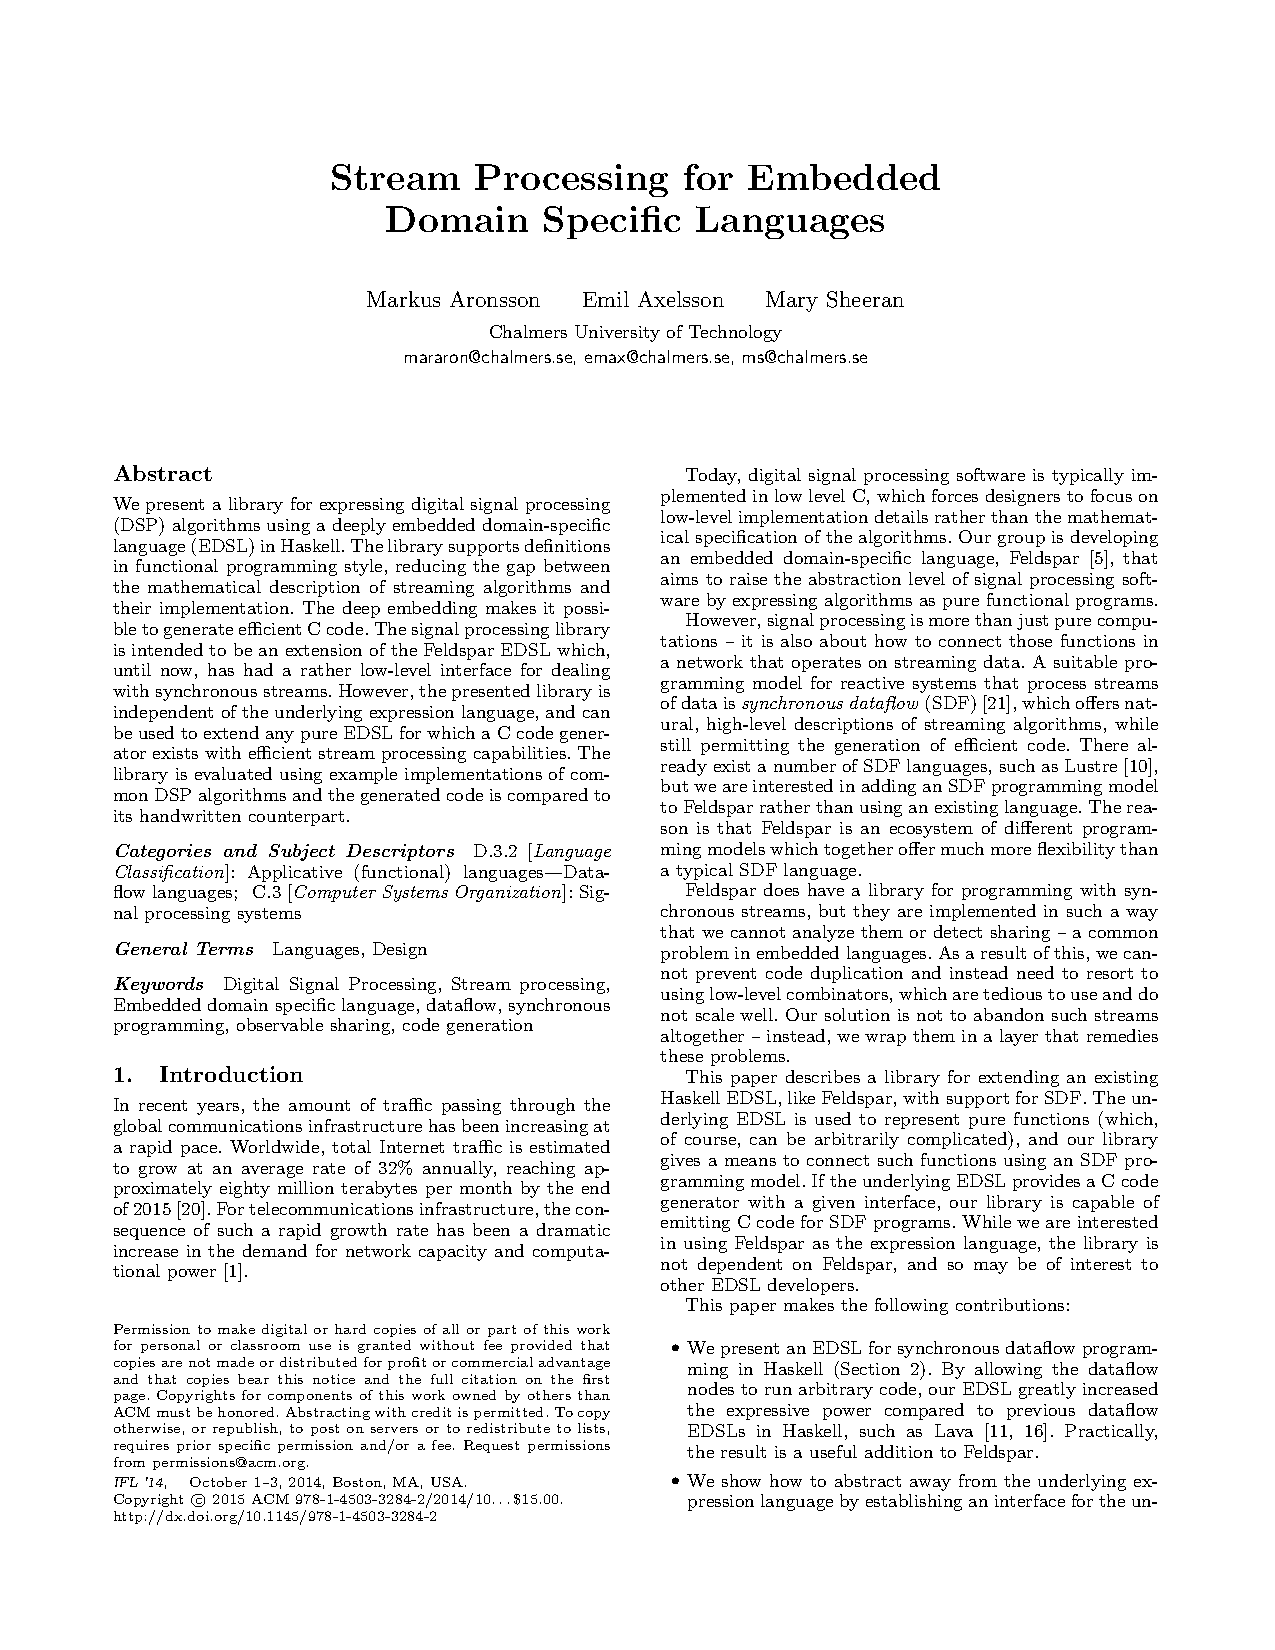
\includepdf[pages=-,width=\paperwidth]{paper-supervisory/paper1.pdf}

\paper{\citefield{aronsson2017}{title}}{\fullcite{aronsson2017}}
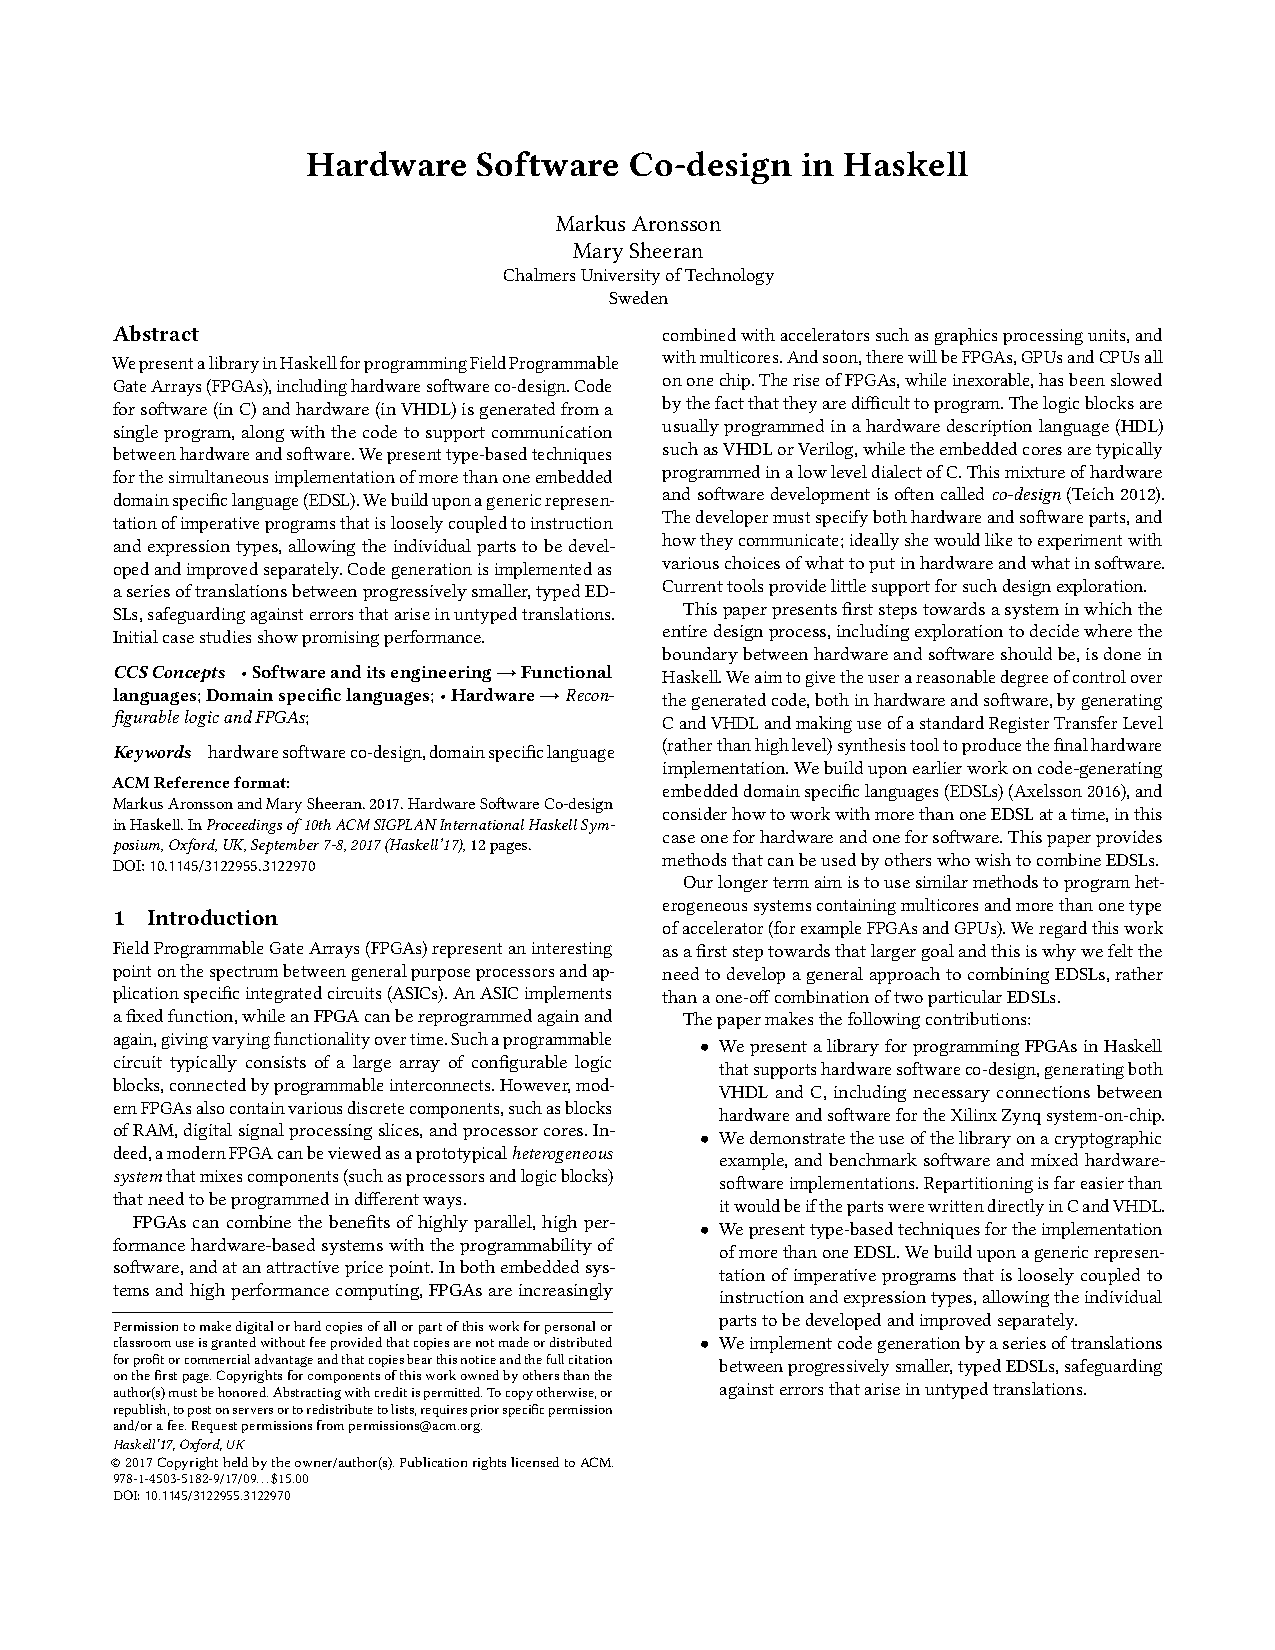
\includepdf[pages=-,width=\paperwidth]{paper-supervisory/paper2.pdf}

\end{document}
